\chapter{Approach}
\label{chap:approach}
This chapter presents the approach of the thesis to describe and
explain the concepts behind the robot memory. It starts with the
goals the robot memory is designed to achieve in
\refsec{sec:goals}. \refsec{sec:formalism} introduces the theoretical
foundation how information can be represented in the robot memory and
how knowledge is transferred into a knowledge based system (KBS). The
concepts of the robot memory's main components are presented in
\refsec{sec:concepts} and \refsec{sec:architecture} gives an overview
of the architecture, which describes in which components the robot
memory is organized and how they interact with each other.

\section{Goals}
\label{sec:goals}
This section presents the design goals of the robot memory. They were
formulated before detailing the concepts used in the robot memory and
define what the robot memory should be capable of. The evaluation in
\refchap{chap:evaluation} refers to these goals to analyze how well
the implementation fullfils them.

\subsection{Flexible Storage and Retrieval:} The main task of
the robot memory is memorizing information of the robot. Memorizing
includes storing newly obtained information, updating it accoring to
changes, removing information that is no longer valid or needed, and
remembering the information by querying it again. Thus the robot
memory has to provide services for storing, updating, removing, and
querying information so that different components can use the robot
memory to provide information, use it as a source, or collaborate
using the same memory.  When the robot memory is queried, it should
only return the information that is asked for. It should be flexible
enough to store any kind of data, information, knowledge, and wisdom
of the DIKW hierarchy in any structure. For example the robot memory
should be able to store world models, perception results and even
large datasets, such as remembered sights of objects.

\subsection{Memory Sharing Between Knowledge Based Systems:}
% original title of the goal: Consistent...
The robot memory has to provide a common memory to allow consistent
memory sharing between multiple components. Thus multiple components have to
use the robot memory at the same time and should have access to common
or each other's information. This should especially allow Knowledge
Based Systems (KBS) to share a common world model, even if the KBS are
of a different type. For example a planner, a world model reasoner,
and an executive should work together using the robot memory as a
common base. This allows combining their specialized strengths
(e.g. generating efficient plans, intuitive world model reasoning, and
robust execution). Furthermore, the robot memory should help avoiding
inconsistencies between KBS by providing a common knowledge base base so that
only one state estimation is necessary.

\subsection{Special Views for Different Components:} Depending on the
application of different components using the robot memory, different
views on the stored data are necessary. For example a planning
components needs another part of the stored data, than a component
learning distributions of object sights. Thus component-specific
filters are necessary. Furthermore, different components need the
stored data in different formats depending on the used programming
language and purpose (e.g. symbolic or spatio-temporal). The robot
memory has to allow defining these views and then accordingly filter
and transform the stored information. Also keys and identifiers, which
might be named differently, have to be translatable.

\subsection{Computation on Demand:}
\todo[inline]{call it 'knowledge' computation?}  To efficiently derive
information only when it is necessary, the robot memory has to provide
computation on demand. This means that some information is not stored
in the robot memory directly, but computed when needed. It allows
accessing information through the robot memory that is otherwise
impracticable to compute and store continuously and for all possible
queries. For example when a component queries the distance of two
objects, it is better to compute the result on demand than to store
all distances between each two objects in the memory and to keep them
updated. Components using the robot memory should be able to provide
knowledge computation functions (\emph{computables}) to the robot
memory. This should add a lot of versatility and expandability.

\subsection{Shared Memory for Multi-Robot Systems:} The robot memory
should be able to distribute parts of the memory in a multi-robot
system. Multiple robots can then share a common world model for
collaboration. This goal is similar to the memory sharing between
knowledge based systems on the same machine with the difference that
the components on a multi-robot system work simultaneously and the
additional difficulty of message loss and keeping consistency. Such a
distributed robot memory is necessary in many multi-robot domains,
especially in the RoboCup Logistics League (RCLL), where the whole
robot team needs to know the world model and what other robots intend
to achieve at the moment.  Distributing the robot memory adds
additional requirements and challenges, especially robustness (e.g. in
the case of robots dropping out), consistency of the memory, and
accessibility so each robot can use the robot memory without large
latices.

\subsection{Spatio-Temporal Grounding:} It is often desirable to ground
stored knowledge based on location and time because this is the
prerequisite for many applications, such as spatio-temporal clustering
and learning distributions (e.g. at which day-times objects can be
found at which positions~\cite{deebul}). Thus the robot
memory has to be able to store knowledge tagged with spatio-temporal
information and consider this information while querying.

\subsection{Triggers:} The robot memory should be able to notify
components about relevant changes in the memory. These notifications
about specified events are called \emph{triggers} and should
automatically be sent after a component registers an event it wants to
be notified about. Events include the appearances of new information
about a specific topic, modifications and deletions of it, as well as
sentences becoming true or queries returning new information.
An example use case that should be supported by the robot memory is
updating reasoner predicates according to changes in the memory.

\subsection{Persistent Storage:} The robot memory should be persistent
to be able to store long-time knowledge and operate over long times,
in which a robot might be restarted. This is necessary in many
domains, such as for domestic service robots and RCLL robots that
might be restarted. Furthermore, it should be possible to distinguish
information that is persistent and information that becomes invalid
after a restart and should be removed.

\subsection{Human Interface and Visualization:} An important factor in the
development of a robotic systems is the accessibility of underlying
components for easier debugging and modeling. Therefore the robot
memory needs to provide an interface for developers to introspect and
modify the state represented in the robot memory. A visualization
would also be desirable to analyze spatio-temporal data efficiently.

\section{Theoretical Foundation}
\label{sec:formalism}
\todo[inline]{emph mit textit oder textbf?}
In this section, we lay the theoretical foundation of the robot memory
and it's integration into knowledge based systems. First, we focus on
the representation of symbolic information as it is used in KBS. Here
we take the PDDL formalism as example. The formal definition of the
robot memory describes how knowledge is represented and how
computables are defined. Because the robot memory is document
oriented, we first define documents and their key-value pairs. This
definition is derived from the specification of the Binary JavaScript
Object Notation (BSON)\footnote{\url{http://bsonspec.org/spec.html}}
used in MongoDB.  Because documents can be nested, we define them by
induction. Unnested documents are defined as follows:
\begin{enumerate}
\item \textbf{Keys} are strings $\mathcal{K} := \Sigma^*$, where
  $\Sigma$ contains all valid characters.
\item  \textbf{Atomic values} are in a countable infinite set $\mathcal{V}_0$ of constants with
  integers, floating point numbers, and strings.
\item \textbf{Unnested key-value pairs:} $\mathcal{P}_0:=\mathcal{K}\times\mathcal{V}_0$
\item \textbf{Unnested documents} are sets of key-value pairs with
  unique keys and thus included in the power set of $\mathcal{P}_0$:\\
  $\mathcal{D}_0:=\{
  d\in\mathbb{P}(\mathcal{P}_0)|
  \forall (k,v),(k',v')\in d , k\neq k' \vee (k,v)=(k',v')
  \}$
\end{enumerate}
Values and documents with a nesting depth up to $n$ with $n>=1$ can be
defined as follows:
\begin{enumerate}
\item  \textbf{Values:} $\mathcal{V}_n := \mathcal{V}_{n-1} \cup \mathcal{D}_{n-1}$
\item \textbf{Key-value pairs:} $\mathcal{P}_n:=\mathcal{K}\times\mathcal{V}_n$
\item \textbf{Documents:}
  $\mathcal{D}_n:=\{
  d\in\mathbb{P}(\mathcal{P}_n)|
  \forall (k,v),(k',v')\in d , k\neq k' \vee (k,v)=(k',v')
  \}$
\end{enumerate}
This yields the set of all \textbf{finitely nested documents}
$\mathcal{D}=\cup_{n\in\mathbb{N}}\mathcal{D}_n$.
The set of all values is $\mathcal{V}=\cup_{n\in\mathbb{N}}\mathcal{V}_n$.
  Infinite nesting and
documents containing themselves are not considered because they can
not properly be mapped into most KBS formalisms.
\\
A \textbf{database} is a finite set of documents $\mathcal{DB} \subset \mathcal{D}$.
%% with unique object
%% identifiers, which are a special key-value pair:
%% \begin{align*}
%% \mathcal{DB} \subset & \{d\in\mathcal{D} | ("\_id",v)\in d\},\\
%% & \text{where } \forall d,d' \in \mathcal{DB} \text{ with } ("\_id",v)\in
%% d \text{ and } ("\_id",v')\in d' , d=d' \vee v\neq v'
%% \end{align*}
\textbf{Queries} are represented by documents $q\in\mathcal{D}$ and
yield a set of documents $r\subseteq\mathcal{DB}$ as result when
executed in a database according a specification (e.g. of
MongoDB~\cite{mongodb}). For example, the query
$\{("object","cup"),("room","kitchen")\}$ yields all documents
containing these key-value pairs, which represent all cups in the
kitchen.
\\
A \textbf{computable} $f$ is a function mapping a query document and
the current state of the database to a set of computed documents:
$$f: \mathcal{D}\times\mathbb{P}(\mathcal{D}) \rightarrow \mathbb{P}(\mathcal{D})$$
The powerset of documents is in the domain of a computable because the
result can also depend on the state of the database (e.g. a computable
calculating the number of objects in the database). For simplicity, we
assume that all sensor data a computable can depend on is also
represented in the database. The component providing the computable
has to ensure that the function is computable and terminates.
%
With these preliminaries, we can now define a \textbf{robot memory} as tuple
of a database~$\mathcal{DB}$ and an ordered set of computables~$\mathcal{C}=\{f_1,...,f_n\}$:
$$\mathcal{RM}=(\mathcal{DB},\mathcal{C})$$
%
The computables are ordered by a priority because a computable with
higher priority can provide documents that are used by a computable
with lower priority. The set of documents \textbf{memorized} by a
robot memory without computables equals the underlying database:
$$mem(\mathcal{(DB,\emptyset)})=\mathcal{DB}$$
For a robot memory with computables the documents memorized are:
$$mem((\mathcal{DB},\{f_1,..,f_n\}))=mem((\mathcal{DB},\{f_1,..,f_{n-1}\})) \cup \bigcup_{d\in\mathcal{D}}f_n(d,mem((\mathcal{DB},\{f_1,..,f_{n-1}\})))$$

To integrate the robot memory into PDDL, we need to define a
\textbf{mapping functions} $map_d$ between documents and predicates, and
$map_v$ between values and terms. As prerequisite, the connection
between key-names in documents and predicates, functions, actions, and their
attributes needs to be defined. Let $\mathcal{R}$ be the \textbf{set
  of predicate symbols}, $\mathcal{F}$ the \textbf{set of function
  symbols}, and $\mathcal{A}$ the \textbf{set of actions
  symbols}, then
%
$$name_{pred}: \mathcal{R} \rightarrow \Sigma^*
\text{ , } name_{func}: \mathcal{F} \rightarrow \Sigma^*
\text{ , and } name_{act}: \mathcal{A} \rightarrow \Sigma^*$$
%
map to the strings used in document keys
(e.g. $name_{pred}(\text{at})="\text{at}"$). To ensure unambiguity,
the $name$ functions should
be injective and their images disjunctive. The function
%
$$ name_{func-atr}: \mathcal{R} \times \mathbb{N} \rightarrow
\mathcal{K}$$
%
maps the attributes in function to a key name. $name_{pred-atr}$ and
$name_{act-atr}$ are defined accordingly
(e.g. $name_{pred-atr}(\text{at},1)="\text{object}"$ and
$name_{pred-atr}(\text{at},2)="\text{room}"$).
\\
Now we can define the mapping of values in documents to terms as
follows. Values that are no sub-documents can be mapped directly to
the corresponding constant:
$$map_f(v)=v, v \in \mathcal{V}_0$$
Otherwise the value is a sub-document, which is mapped to a function term:
\begin{align*}
  map_f(d)= &\text{ }f(map_f(v_1), ..., map_f(v_n)), \text{ iff } f \text{ is a n-array function in } \mathcal{F},\\
  &("function", name_{func}(f))\in d,
  \forall i \in \{1..n\} (name_{func-atr}(f,i), v_i)\in d\\
  map_f(d)= &\text{ } nil_f, otherwise\text{~~~~~~~~~~~~~~~}
\end{align*}
where $nil_f$ is a new constant used for not mappable documents.
Similarly documents can be mapped to predicates as follows:
\begin{align*}
  map_p(d)=&\text{ }p(map_f(v_1), ..., map_f(v_n)), \text{ iff } p \text{ is a n-array predicate in } \mathcal{R},\\
  &("predicate", name_{pred}(p))\in d,
  \forall i \in \{1..n\} (name_{pred-atr}(p,i), v_i)\in d\\
  map_p(d)=& \text{ }nil_p, otherwise\text{~~~~~~~~~~~~~~~}
\end{align*}
For example is
\begin{align*}
map_p&(\{("predicate", "at"),("object", "cup"),("room",
"kitchen")\})\\
&= at(map_f("cup"), map_f("kitchen")) = at(cup, kitchen) \text{.}
\end{align*}
This theoretical foundation of the robot memory and the mapping of
queried documents into predicates is the basis for the generation of
PDDL problem descriptions. The direction from PDDL back to the robot
memory is limited on storing the resulting plan found by a
planner. The plan $\mathcal{L}$ is an ordered sequence of
parameterized actions
$$\mathcal{L}=(a_1(v_{1,1},v_{1,2},...,v_{1,k_1}),a_2(v_{2,1},...,v_{2,k_2}),...,a_j(v_{j,1},...,v_{j,k_j})) \text{.}$$
where $a_i$ is an action with $k_i$ parameters and $j$ is the length
of the plan. The resulting plan is then maped into a document
containing the actions as subdocuments:
\begin{align*}
  map_L(L)=&\{("plan", "success")\} \cup_{i \in \{1..j\}}\{(n_i, map_a(a_i))\} \text{,}
\end{align*}
where $\mathcal{L}$ is defined as above, $n_i$ is the number $i$ as
string, and $map_a$ maps a parameterized action to a subdocument,
similar to the inverse of $map_f$:
\begin{align*}
  map_a(a_i(v_{i,1},...,v_{i,k_i}))= &\{("action", name_{act}(a_i))\} 
\cup_{m \in \{1..k_i\}}\{(name_{act-atr}(a_i,m), v_{i,m})\}
\end{align*}
If the planner can not find any plan, the result is mapped to the
document ${("plan", "fail")\}$.

For the knowledge representation in the robot memory and the
integration into PDDL, the closed world assumption is kept. Thus if
there is no document $d\in mem(\mathcal{RM})$ so that
$map_p(d)=p(v_1,v_2)$, $p(v_1,v_2)$ is known to be false.

Although it is not included in the theoretical foundation focused on
PDDL, the robot memory can also map spatio-temporal information into
other systems such as CLIPS and C++. Here, the documents in
$mem(\mathcal{RM})$ are not directly mapped into the used
representation of CLIPS (e.g. as facts) or C++ (e.g. as
variables). Instead, there are functions for querying, which yield a
set of documents, and functions to receive the value of a key-value
pair in different types. Furthermore, there are functions to build
documents and queries iteratively pair-by-pair and inserting,
updating, and removing removing.

\section{Robot Memory Concepts}
\label{sec:concepts}
This section presents the concepts behind important aspects of the
robot memory in more detail. These concepts are computables for
computation on demand, trigger for notifications about events in the
database, interfaces of the robot memory to knowledge based systems,
and the distribution of the robot memory in a multi-robot system.

\subsection{Computables}
\label{sec:computables}
Computables are functions that provide information or knowledge on
demand. Thus the information provided by the computable is not stored
directly in the database, but will be computed when some application
asks for it. The robot memory manages the list of available
computables and checks which coputables need to be called to answer a
query. The concrete computables are provided by other components. For
example, a vision component can register a computable that computes
which objects are currently visible at which position. We use
computables in our robot memory for three main reasons:
\begin{itemize}
\item Computables ease knowledge based systems to deal with
  complex data. By using the robot memory interface, KBS can access
  functions that are provided by other components and compute
  information that is difficult or impossible to compute inside the
  KBS. For example, a KBS using a computable can ask for a closest
  object even if the KBS does not support arithmetic operations. This
  way, KBS can bypass some expressiveness and complexity limits.

\item Computables decrease the computational effort that is necessary
  to collect the information contained in the robot memory. For some
  problems, it is not appropriate to continiously compute and store
  the results in the robot memory. Rather, it is better to compute the
  results on demand only when it is neccessary and only with the
  parameters needed at the moment. One common example of these
  problems in the robotics context is perception, which can be
  computationally costly and might be needed only rarely (e.g. the
  detection of objects on a table is only neccessary when the robot is
  searching for something on a table). Another set of problems that
  are well suited to be solved by computables deal with values
  changing rapidly over time and a wide variety of possible
  parameters. For example the transformation result of object
  coordinates change rapidly while the robot is moving and there might
  be many objects that might be transformed to the different frames
  used by the robot. Thus it is impractical to compute and store the
  positions of all objects in all frames in the robot memory and keep
  them updated. It is a better idea to provide the transforms in the
  robot memory as computable so only the transformation only needs to
  be done when it is needed and for the subset of objects that are
  currently needed.

\item Computables simplify hybrid reasoning by transforming
  spatio-temporal information into symbolical information and vice
  versa. Becasue of the KBS interface and the decreased computational
  effort mentioned in the previous two reasons, computables are well
  suited to simplify dealing with hybrid information in KBS. For
  example computables can provide a KBS with the infomation in which
  room the robot is based on the current 3D position of the robot
  stored in the robot memory. An example for the transformation of
  symbolical to geometric information is finding a free position on a
  table for a planner action specifying to place an object on a table.
\end{itemize}

According to the formal definition of computables in
\refsec{sec:formalism}, computables are a function taking a query as
input and returning a set of computed documents. Furthermore,
computables can also use the documents currently provided by the robot
memory as a basis for the computation (e.g. to transform the
coordinates writen in the robot memory to another frame). The robot
memory has to decide when the function of a computable needs to be
executed given an asked query. To decide this, each computable also
contains a definition which queries can be answered by
it. Furthermore, each computable has a priority defining in which
order computables are executed if a query can be answered by multiple
computables. This allows computables to depend on other the results of
other computables. The documents resulting from a computable are
temporily added to the robot memory so that a query can be evaluated
on computed information and persistent information in the database of
the robot memory.

\subsection{Trigger}
Trigger are mechanisms that invoke a callback function if a specified
event occurs in the robot memory. The main application of triggers in
this thesis is to notify components using the robot memory about
changes of the stored information. Furthermore, they can be used to
check for more complex conditions each time a relevant document in the
robot memory changes. Triggers consist of a definition of the event...

mostly new doc of some type, changes, deletions
notification about changes in the rm
registration with definition of event
notifications
no trigger on not demanded computables
avoids polling in application
keeps world model up to date
can be used to send messages
rm manages and checks

\subsection{Knowledge Based System Interface}
\subsection{Multi-Robot Synchronization}

\section{Architecture}
\label{sec:architecture}
This section presents the architecture of the robot memory and
explains its design considerations. It shows how the intended
functionality is organized in smaller components and how these
components interact with each other. The architecture contains
standard concepts of software engineering, most importantly a layered
architecture, functional abstraction, and data
abstraction~\cite{software-architecture} to allow
reusability and adaptability to changing requirements and use cases.
%% functional abstraction,
%% %% (e.g. of the different processes happening during storing and
%% %% querying)
%% and data abstraction.
%% %%  (e.g. of stored knowledge which is
%% %% more specialized internally than visible from a using
%% %% application)
\reffig{fig:arch} shows the architecture of the robot
memory and is explained in the following.
\begin{figure}
  \centering
  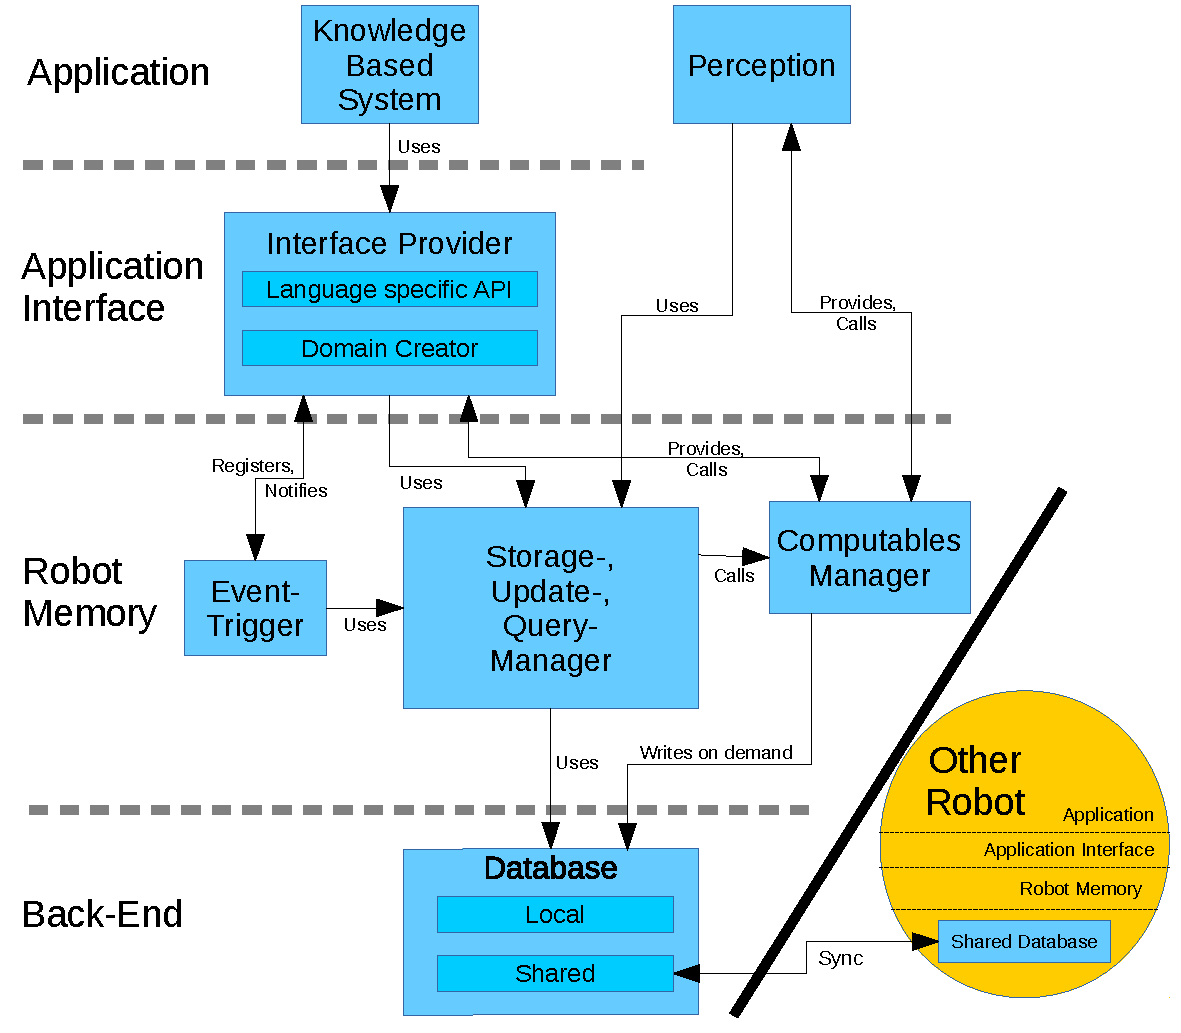
\includegraphics[width=\textwidth]{architecture.pdf}
  \vspace{-5mm}
  \caption[Software architecture of the Robot Memory]{Software architecture of the Robot Memory}
  \label{fig:arch}
  \vspace{-5mm}
\end{figure}
The architecture organizes all components into four layers: Back-End,
Robot Memory, Application Interface, and Application. The Back-End
contains databases for storing knowledge and executing queries. There
is a local private database, which is private to the robot, and a
shared database distributed between multiple robots using the same
architecture. This distribution can utilize the replication features
of the database. The Robot Memory-layer contains the central functions
that distinguish the robot memory from a pure database. It contains
the operation manager, which is used to execute store, update, query,
and delete operations. The operation manager is an intermediate
component that realizes most of the robot memory's functionality by
modifying and enhancing queries, storage, and update requests before
applying them to the database. The operation manager also handles the
database interaction and distinguishes if operations should be
executed on the local or the shared database.  If a query asks for
knowledge provided by a computable, the operation manager forwards it
to the computable manager. The computable manager keeps a record of
which computable is provided by which application and requests the
demanded computation. The component responsible for triggers
receives and manages registrations of applications that want to be
notified in the case of an event. It listens to logged changes in the
databases to check if events happen and notifies applications
accordingly. Additionally the operation manager can initialize the
robot memory (e.g. to setup the world model for a new RCLL game).
Between the robot memory and a planner or reasoner components, there
is the Application Interface layer. For each KBS, it includes an
Interface Provider component, which makes the function of the robot
memory available to the KBS and the special programming language
used. It is not necessary for components that can directly use the
interface of the robot memory (available in C++). The responsibilities
of the interface provider also include transforming query results in
the appropriate format used by the KBS and eventually renaming
key-names if they have be mapped to match the names used in the KBS
model. Because languages and concepts of knowledge based systems can
be very different, each KBS needs a separate Interface Provider. The
Interface Provider can also contain a domain creator, which creates an
initial state (e.g. a problem definition or initial fact base) from a
template and additional knowledge resulting from queries. Finally the
Application layer contains all components using the robot memory
either through the Interface provider or directly through the robot
memory interface. KBS can also register triggers through their
interface provider and perception components can provide computation
functions for computables. The sources and consumers of knowledge
stored in the robot memory are the applications using it. The ordinary
data flow starts in the application requesting storage, modification,
or querying of knowledge (over the language specific interface). The
operation manager forwards the request enhanced with management
information to the database. For queries, the result is transferred
back on the reversed path of the query request. For computables, the
only difference in the data flow is the knowledge computation before
executing the query in the database. The operation manager
additionally initiates the knowledge computation via the Computables
Manager, which forwards the query to the application providing the
specific computable. The documents resulting from the computable are
then stored by the computables manager in the robot memory, where it
is queried afterwards.
\todo[inline]{add dataflow examples as UML sequence diagram?}
